\chapter{Background}

In this chapter we describe model architectures, concepts and training
methodologies our work uses.


\section{Text embedding}

To allow neural networks to process text, each continuous piece of text is
mapped to a series of vectors that represent it. This mapping and its result is
called an embedding. Traditionally we would split the input text
to sub-words and allow the network to change their embedding arbitrarily to
solve some end task. Example of such task is sub-word prediction, where the
network guesses masked-out sub-word.

In our work we train a network to map a long piece of text to a single vector.
As the size of the embedding is limited, we expect the network to effectively
compress the input. In this work our aim is not to reconstruct the input from
the embedding, but rather to capture both the structure and meaning of the text.

\section{Sparse attention}

Traditional Transformer encoder uses full-attention, which means that every
token can interact (or attend) to any other token. This type of attention
creates quadratic number of interactions to input length and therefore also
quadratic time and space complexity. This seriously limits use of transformers
for longer inputs even with efficient cuda kernels (TODO: really? Citation
needed). To overcome this issue, interactions between some tokens are ignored.
Such type of attention is called sparse.

TODO: My graphic of attentions

\begin{figure}[h]
    \centering
    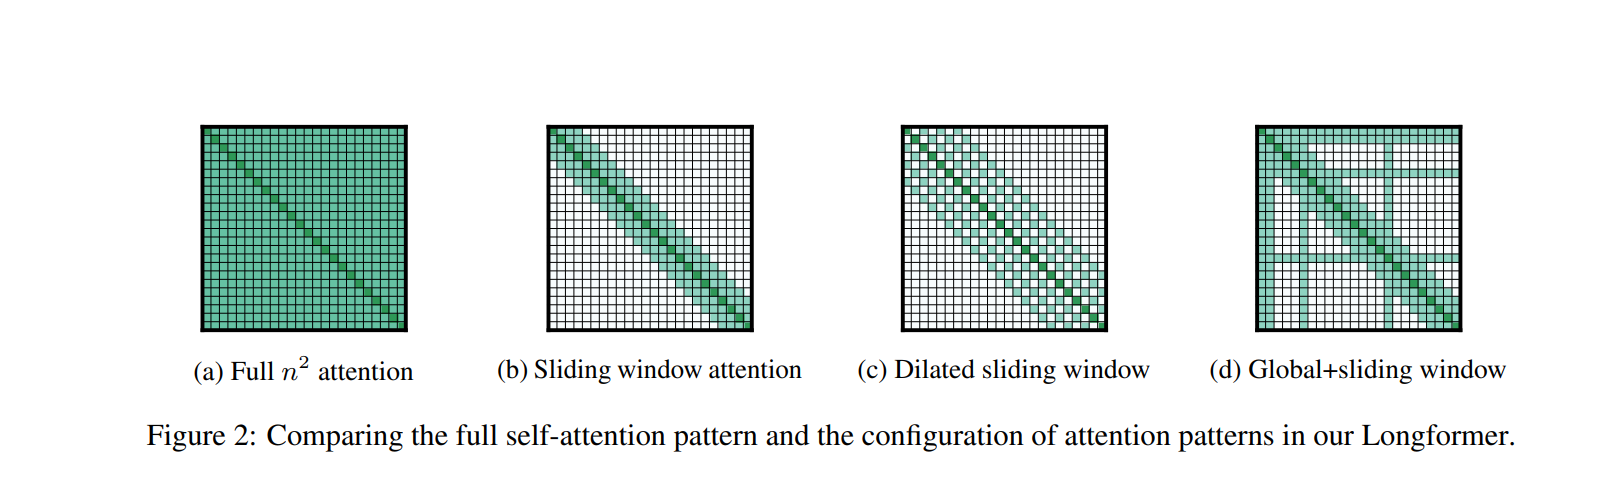
\includegraphics[width=0.9\textwidth]{./img/longformer_attention.png}
    \caption{Longformer attention matrix.\label{fig:longformer_sparse_att}}
\end{figure}

Sparse attention can have different designs but they are usually composed of
several types of mechanisms (such as sliding window, global, random -- I can
write more about this).

\section{Contrastive loss}

Contrastive losses are types of losses which compare several model's outputs to
each other and based on this comparison they compute a value, which can be used
as a loss. Contrastive loss is often used when the model's goal is to
understand and distinguish different inputs. In this setting, we would penalize
the model if the representations of similar inputs are far apart or if the
representations of different inputs are close. Similar inputs are called
positives, whereas distinct inputs are called negatives.

When no supervised information about the similarity of a pair of inputs is
available, we can use in-batch outputs as negatives. Here we automatically
assume that all our inputs are distinct and that the model should distinguish
between all of them.
